\section{PASS Discrimination}
    The use of squeezed states instead of coherent states can allow to overcome the limits
    of precedent systems. The representation of a noisy squeezed state is given in 
    \ref{squeezedStates}. In this section the advantages of the use of squeezed states 
    without photon addition, are initially discuss; then the effect of the photon addition
    in a quantum OOK and BPSK systems are evaluate.

    \subsection{Squeezed states discrimination}
        At first, the effect of squeezing, whithout photon addition and thermal noise, on the
        performance are assessed. As for PACS systems, it can be useful to define the mean 
        number of photon $n_p$ in a squeezed state, that is given by
        \begin{equation}
            n_p(\mu,r) = \absolutevalue{\mu}^2 + \sinh{r}^2;
        \end{equation}
        where $\mu$ is the amplitude of the starter coherent state and the squeezing factor
        is $\zeta = r e^{i\theta}$. The minimum value of $n_p$ is given by $n_p(0,r) = \sinh{r}^2$.

        \begin{figure}[ht]
            \caption{MDEP of squeezed state BPSK system.\\
            $N=30$, $\bar{n}=0$, $\theta=\pi$, $p_0=p_1=1/2$}
            %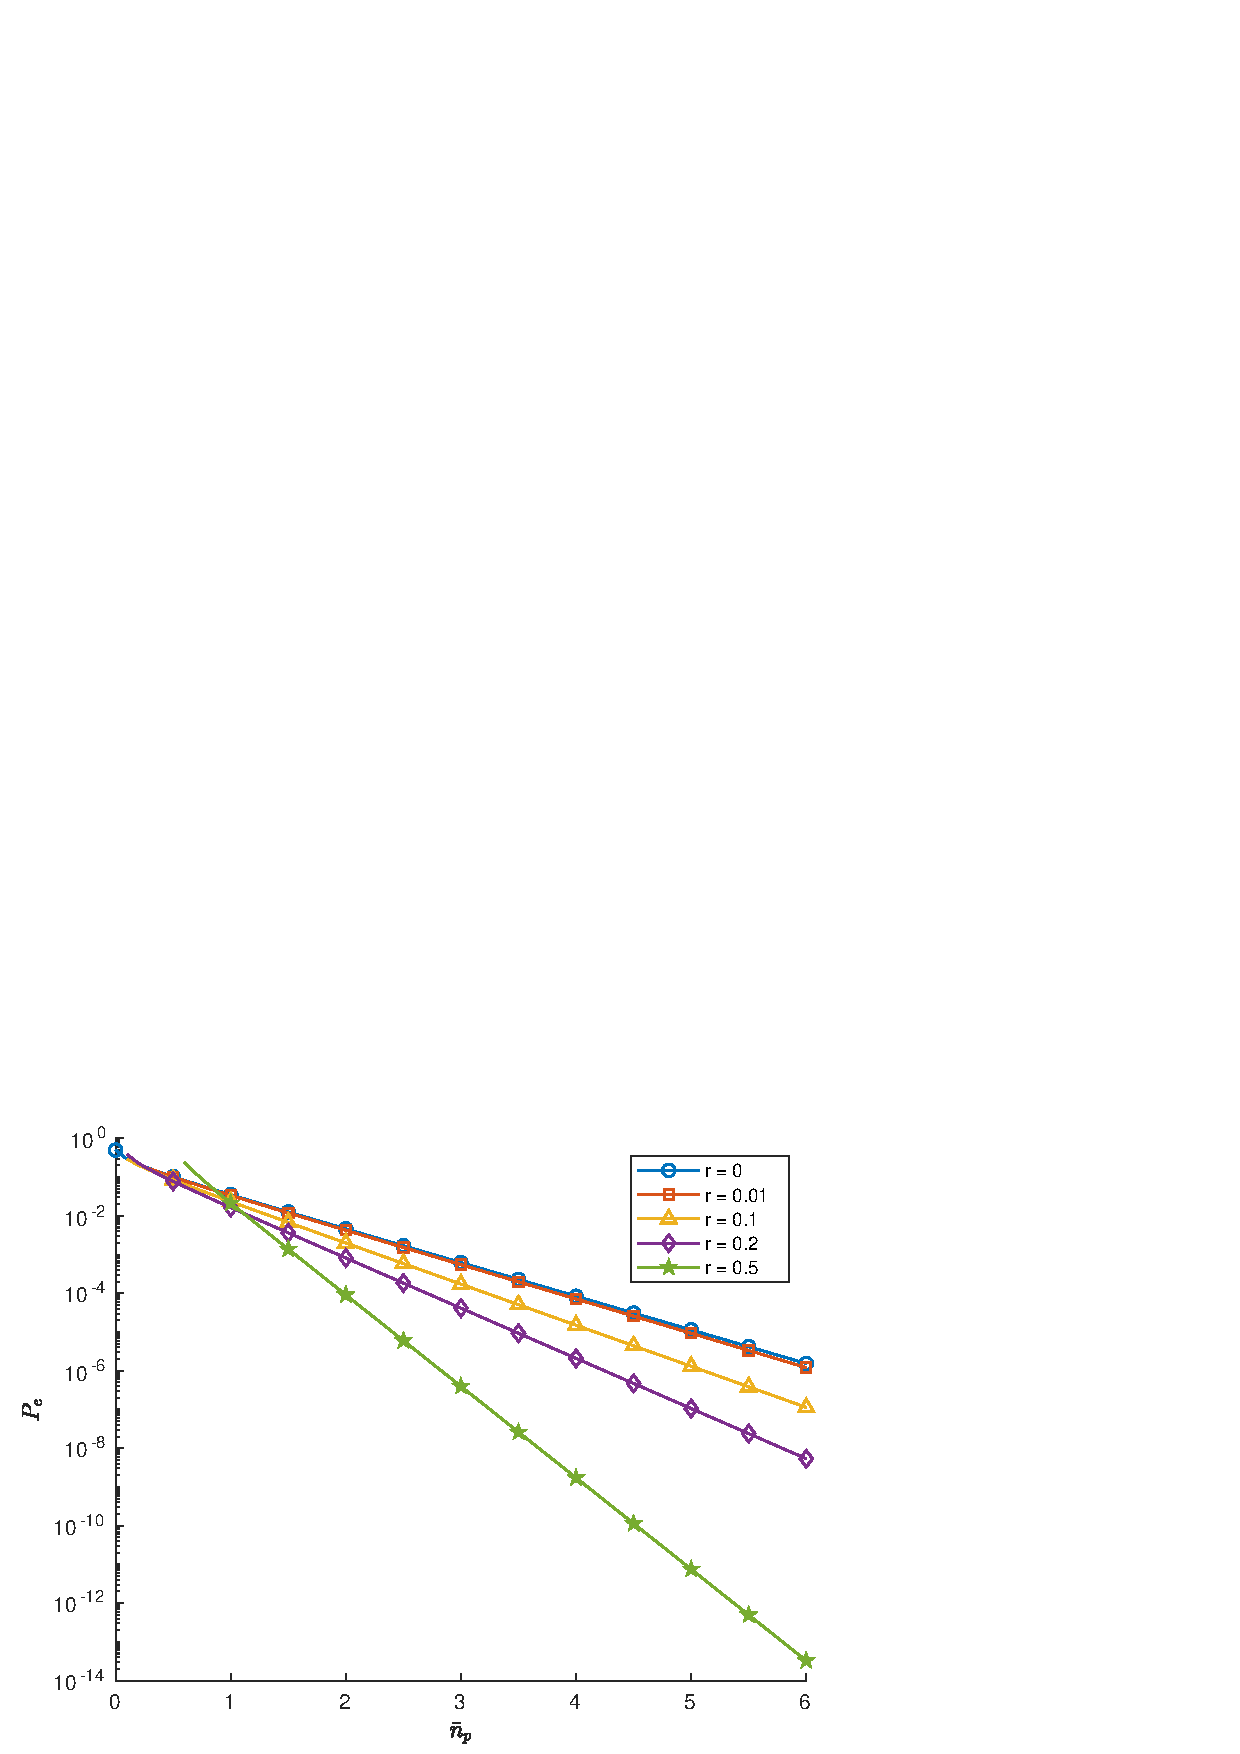
\includegraphics[width=0.75\textwidth]{fig3.5.pdf}
            \label{fig:3.5}
        \end{figure}
        For a quantum squeezed states BPSK system, the MDEP, obtained with the Helstrom bound 
        \ref{eq:HelstromBound}, is plotted in figure \ref{fig:3.5} in function of $\bar{E}$,
        i.e the mean energy of the system (given by the sum of $n_p$ for each state), with:
        $\theta=\pi$, $N=30$, equiprobable symbols and $\bar{n}=0$.

        It can be notice that the optimal configuration of $r$ depends from the energy in the 
        system. For low energy levels the squeezing has not a positive effects.